\section{Server}
Na serveru běží dva programy. Jeden z nich čeká na informace od uživatele, které zpracuje a uloží do databáze. Druhý se stará a webovou stránku.

\subsection{Databáze}
Pro ukládání informací o hráčích jsem vybral databázi SQLite, protože jsem nikdy dříve databáze nepoužíval a SQLite mi přišla jako jednoduchá a pro moje potřeby dostatečně rychlá možnost.

Nejprve jsem si vytvořil databázi s jedním stolem "users", do kterého ukládam ID hráče, dále jeho přezdívku a nakonec jeho highscore.

Ve chvíli, kdy přijdou na server informace od hráče, program uloží do databáze informace a databázi si srovná sestupně podle highscore, vezme ID prvních 10-ti nejlepších hráčů a uloží je do souboru JSON. Z tohoto souboru JSON dále druhý program vezme IDs a podle nich vytvoří tabulku nejlepších hráčů, která je dostupná na webové stránce.

\subsection{Webová stránka}
Pro vytvoření webové stránky jsem použil knihovnu FastAPI, která se stará o zpracovávání requestů. Při otevření webové stránky na endpointu "/", Vám program pošle HTML s tabulkou top deseti hráčů.

V případě, že některý hráč nemá skóre, aby se umístil v tabulce nejlepších 10-ti, může přes vyhledávač vyhledat svou nebo kteroukoliv přezdívku. V moment co vyhledáte přezdívku, server se podívá do databáze a pokud najde hráče s touto přezdívkou, tak Vás přesměruje na tabulku skóre konkrétního hráče a pokud přezdívka neexistuje, tak server vrátí HTML s hláškou, že hráč nebyl nalezen. 

\begin{figure*}[ht!]
    \centering
    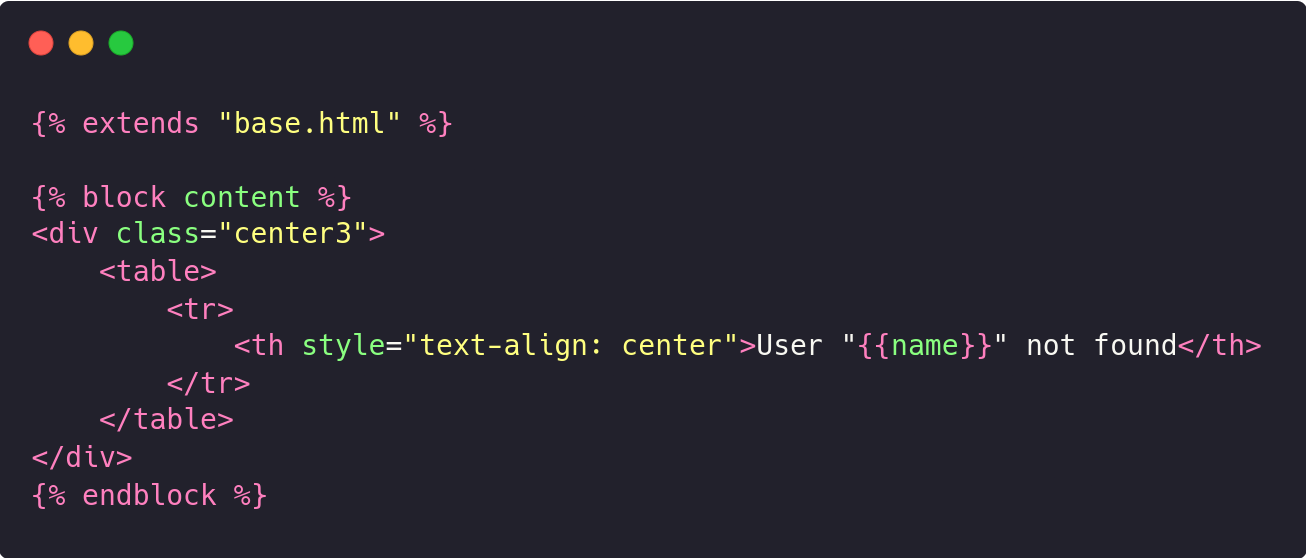
\includegraphics[scale=0.3]{images/carbon (4).png}
    \caption{Extendování html}
\end{figure*}

Pro pracování s HTML jsem použil Jinja template. Díky kterému jsem si mohl vytvořit base HTML, který jsem extendoval a přidával prvky podle potřeby. Jinja také umožňuje předávání proměnných z backend kódu přímo do HTML, díky čemu jsem mohl vytvářet tabulku s informacemi o hráčích přímo z databáze. 


\begin{figure*}[ht!]
    \centering
    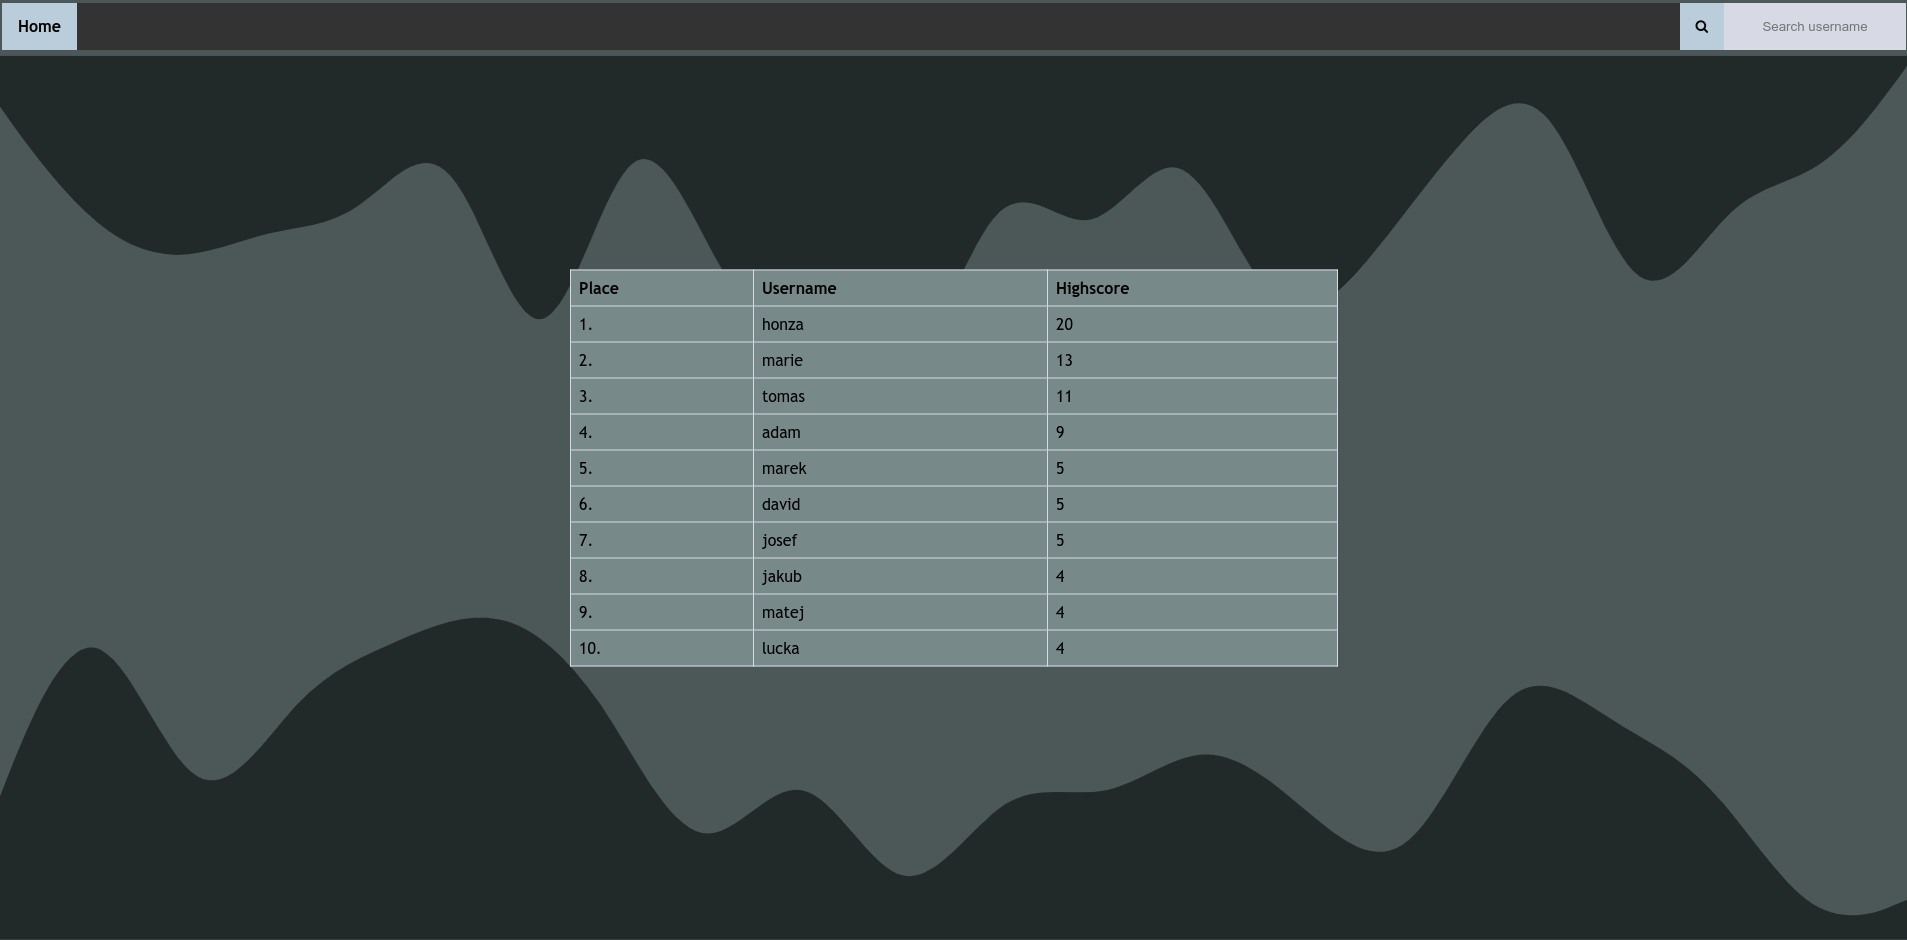
\includegraphics[scale=0.2]{images/Screenshot from 2022-04-27 20-57-42.png}
    \caption{Webová stránka}
\end{figure*}